Three \acrshort{hmi}s have been configured and programmed as control sources for the lolly machine. This chapter provides detail into \acrshort{hmi} development. All \acrshort{hmi}s communicate with the \acrshort{plc} through Modbus \acrshort{tcpIp}.

\section{Siemens HMI}
    A KTP600 Siemens \acrshort{hmi} is the main control source and is permanently mounted to the front of the machine. The KTP600 is a touch screen device accompanied by six push buttons.  This \acrshort{hmi} serves as a setup and diagnostic tool for operators as well as an interface for machine users on open days. With many users being children, a main design consideration was that user screens needed to be functionally simplistic with a `fun' feel. The layout of the screens will be discussed further in Section \ref{sec:hmiScreens}. Programming the KTP600 was done using \acrfull{tia} Portal by Siemens.

        \begin{figure}[H]
            \centering
            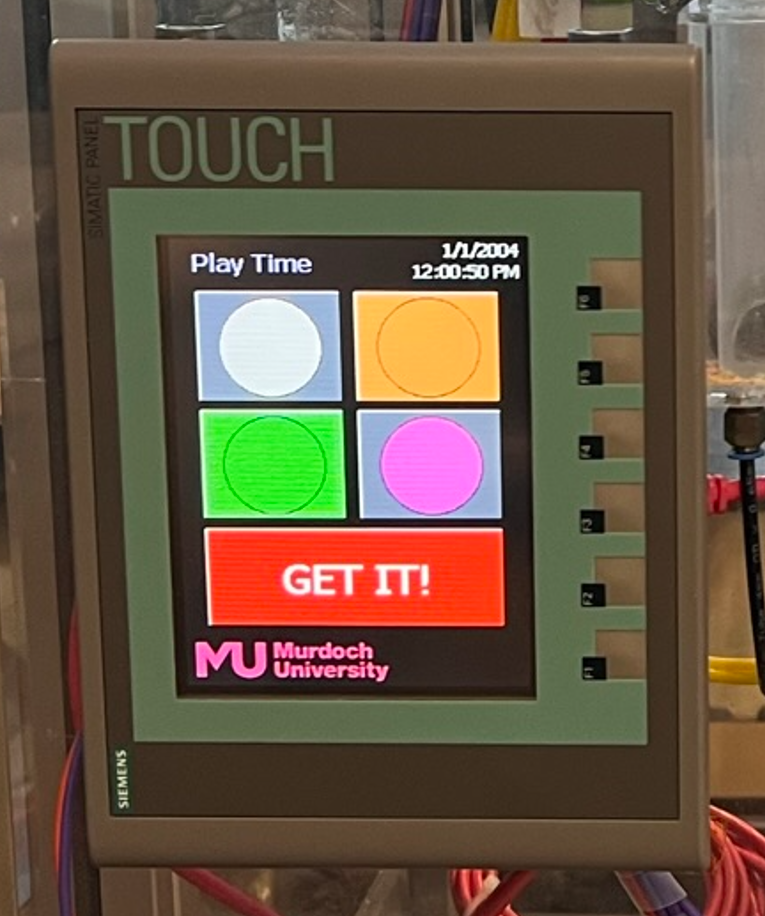
\includegraphics[width = 0.45\textwidth]{2_images/hmiInstalled}
            \caption{The Siemens HMI showing the Play screen.}
            \label{fig:hmiInstalled}
        \end{figure}    
    
    \subsection{Configuration}
        \subsubsection{Modbus Communication}
            To allow communication between the \acrshort{hmi} and the \acrshort{plc}, a connection must be added and configured within the \acrshort{hmi}. Figure \ref{fig:modbusHmiConfig} shows the configuration for the Modbus connection between the \acrshort{hmi} and \acrshort{plc}. Once a Modbus connection is added and configured, \acrshort{hmi} tags need to be defined. \acrshort{hmi} tags are address links between the \acrshort{hmi} and the \acrshort{plc}. Objects (buttons, indicators, etc) on the \acrshort{hmi} screens are linked to tags with read and/or write access. 
            
        \begin{figure}[H]
            \centering
            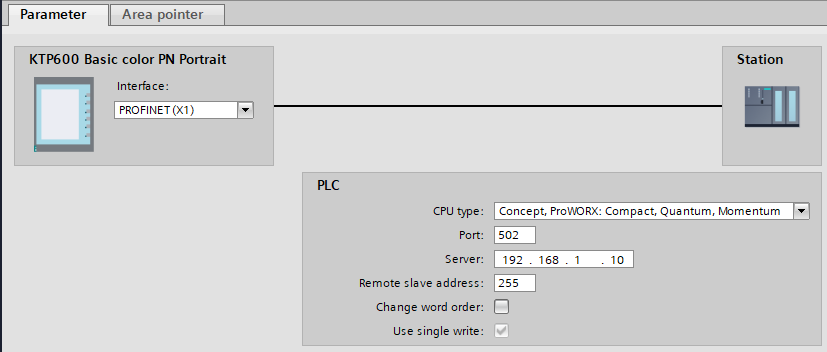
\includegraphics[width = 0.5\textwidth]{2_images/modbusHmiConfig}
            \caption{Configuration settings for a Modbus connection within the Siemens HMI.}
            \label{fig:modbusHmiConfig}
        \end{figure}        
        
        \subsubsection{Alarms}
            Two alarm Words transmitted from the \acrshort{plc} provide the \acrshort{hmi} with 21 different discrete alarms where each bit within each word is associated with a different alarm. Discrete alarms are made up of a trigger tag and a trigger bit. The tag is the alarm Word and the trigger bit is the index of the bit within the alarm word. This is illustrated in Figure \ref{fig:hmiAlarms}.

        \begin{figure}[H]
            \centering
            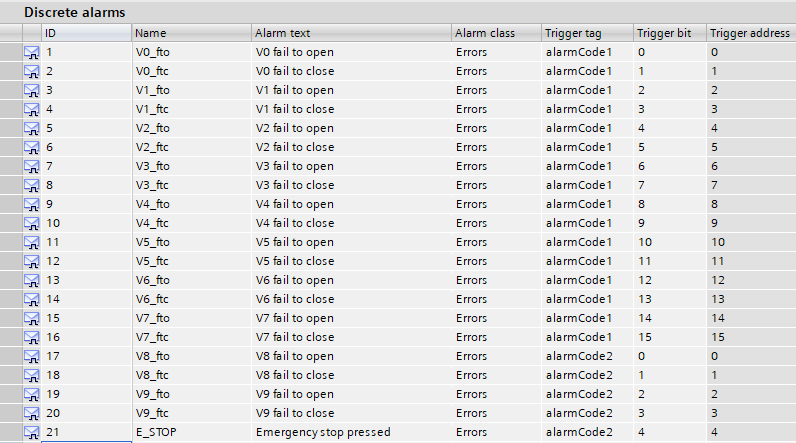
\includegraphics[width = 0.6\textwidth]{2_images/hmiAlarms}
            \caption{Alarm configuration of the Siemens HMI.}
            \label{fig:hmiAlarms}
        \end{figure}    

         When an alarm occurs, a popup containing alarm details will appear on the \acrshort{hmi}. To reset the alarm, the F1 (reset) button must be pressed. To clear the popup the ! button must be pressed. Figure \ref{fig:hmiAlarm} provides an example of what an alarm looks like on the \acrshort{hmi}.

        \begin{figure}[H]
            \centering
            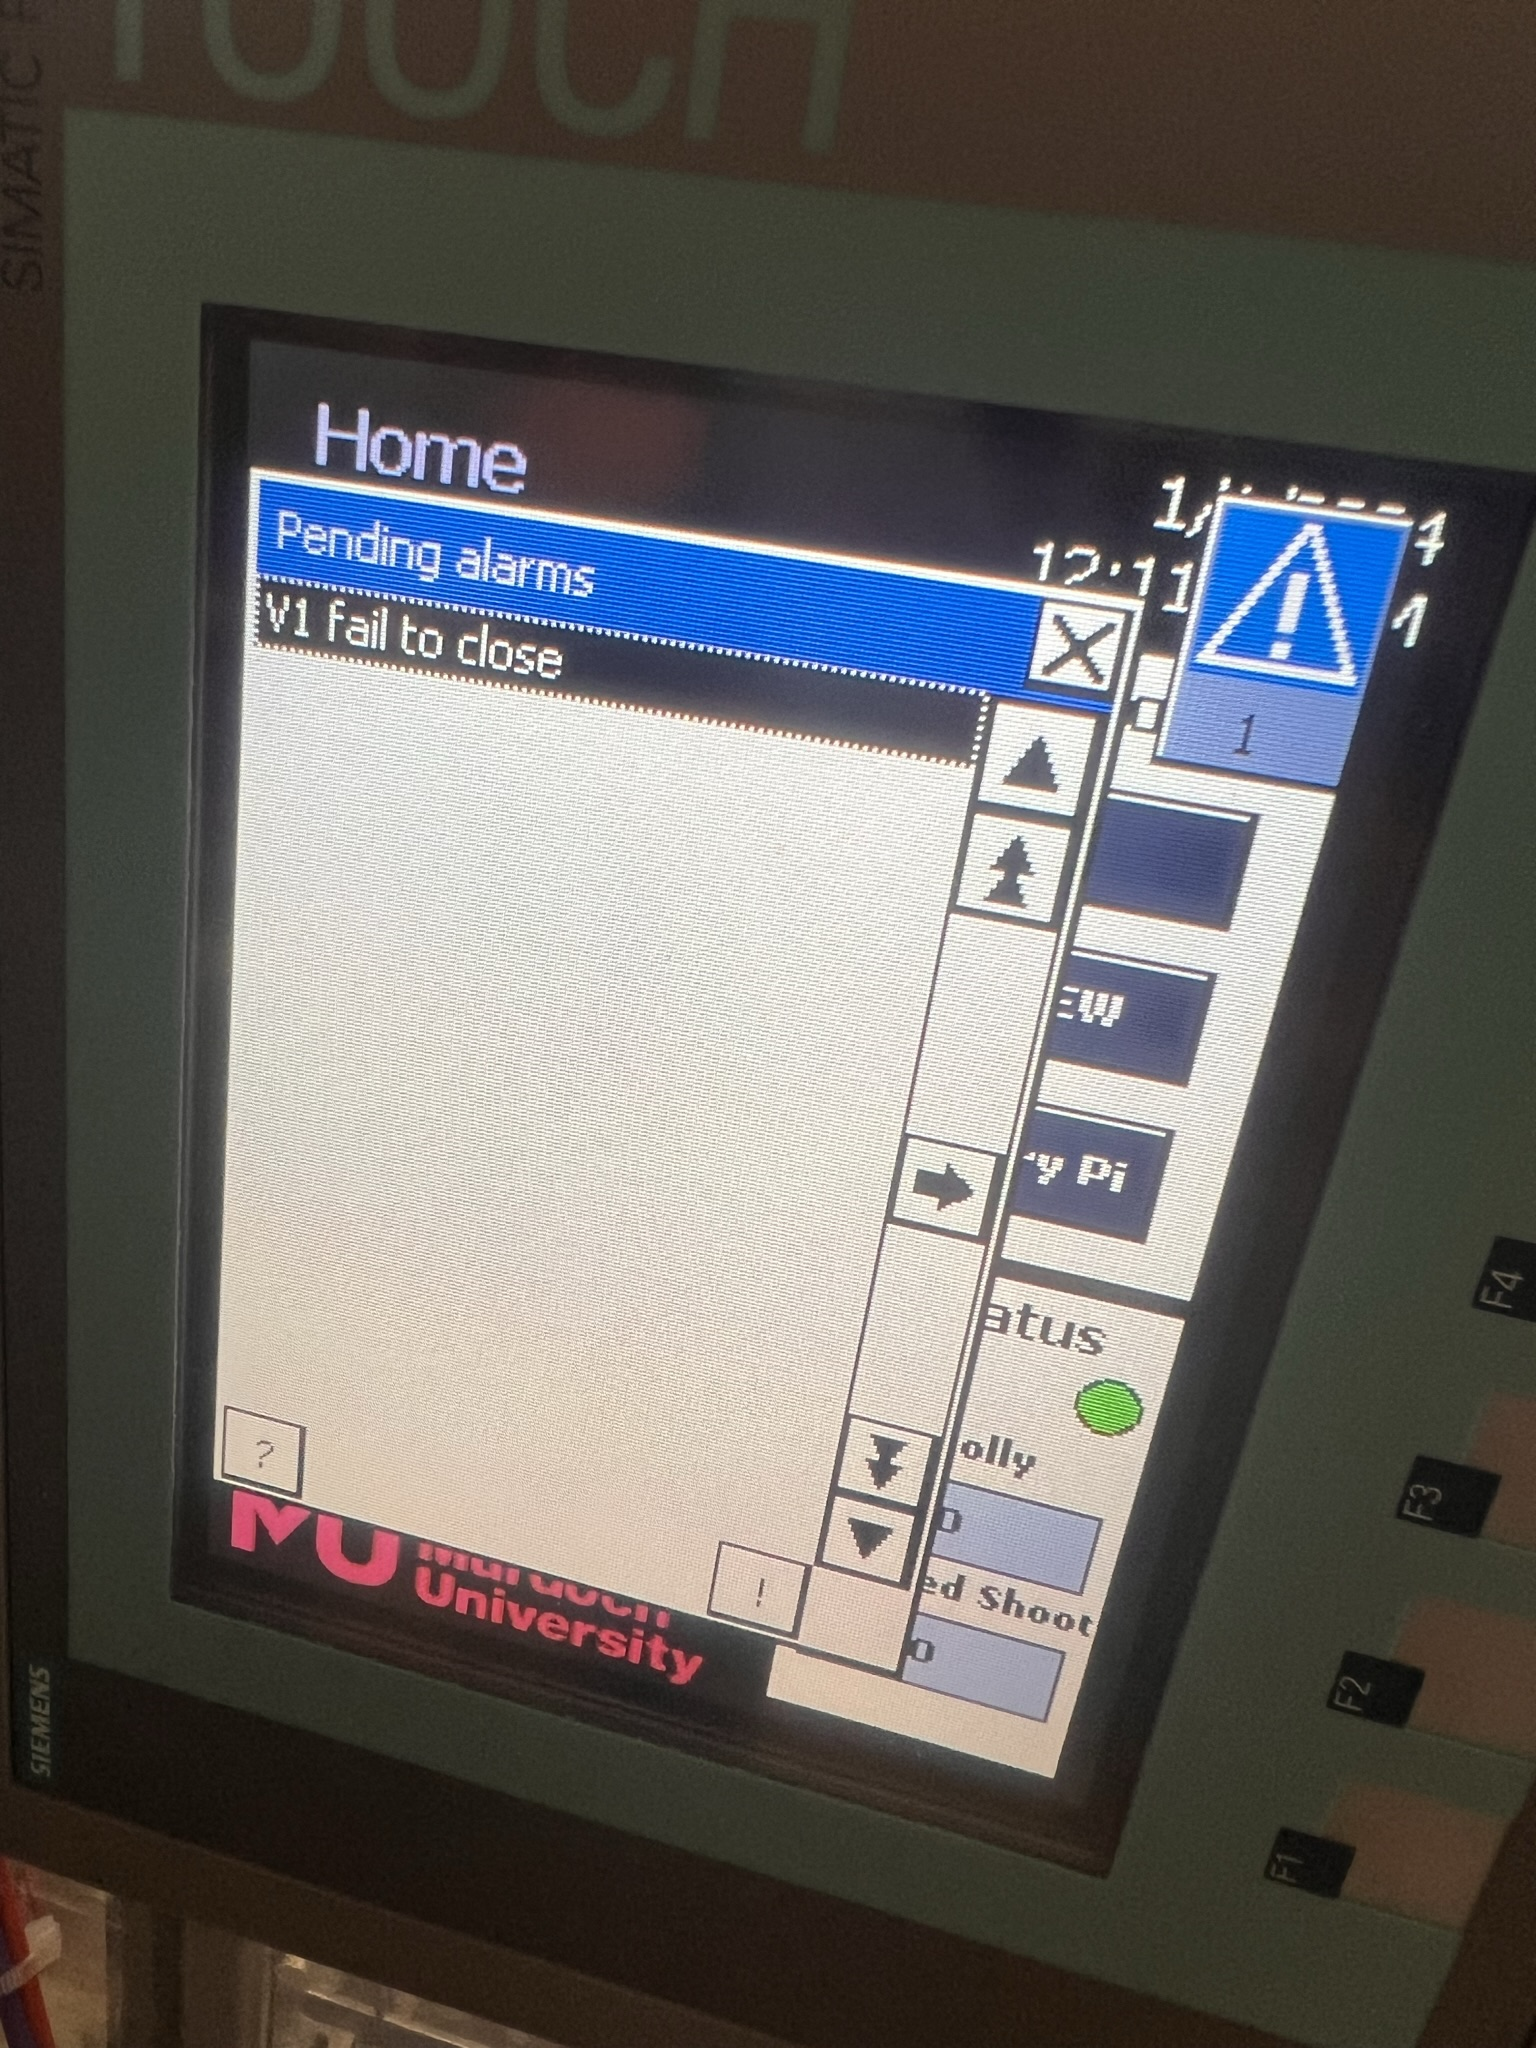
\includegraphics[width = 0.3\textwidth]{2_images/hmiAlarm}
            \caption{V1 fail to close alarm.}
            \label{fig:hmiAlarm}
        \end{figure}  
            
        \subsubsection{Heart Beat}
            The heartbeat from the Siemens \acrshort{hmi} is produced by a status word which Siemens refer to as the coordination area pointer. The second bit of the coordination area pointer is the `Life Bit' which is used as the heartbeat signal to the \acrshort{plc}. The coordination area pointer is linked to a Modbus address within the configuration connection.
            The startup bit and operation mode bits are not used within this project. 

        \begin{figure}[H]
            \centering
            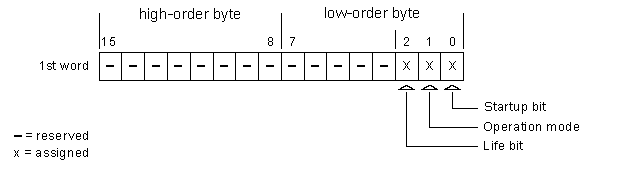
\includegraphics[width = 0.6\textwidth]{2_images/hmiCoordination}
            \caption{Coordination area pointer bit assignment\cite{tiaManual}}
            \label{fig:hmiCoordination}
        \end{figure} 
            

    \subsection{Screens} \label{sec:hmiScreens}
        Four screens provide user interfaces for configuration, diagnostics and general users who just want lollies. Six F keys on the right of the screen have been configured with various functions these are as follows:

        \begin{description}

        \item[F1:] Go to home screen
        \item[F2:] Go to play screen
        \item[F3:] Spare 
        \item[F4:] Spare
        \item[F5:] Toggle sorting program
        \item[F6:] Reset/ acknowledge alarms
        
        The `F' keys have been intentionally left unlabeled to discourage younger users from pressing the buttons. 
        Operation of the Siemens \acrshort{hmi} is outlined in the user manual in Appendix \ref{app:userGuide}
        
        \end{description}

        \subsubsection{Play}
        The play screen (Figure \ref{fig:hmiPlay}) has been specifically designed for users on open days. The main design consideration for this screen was to make it as simplistic as possible to allow operation from young users. 
        To use the play screen, the machine must be enabled in automatic mode. This screen is linked to the dispensing function of the machine.  The play screen can be accessed from the home screen by pressing the `Play' button or by pressing F5. 
        
        \begin{figure}[H]
            \centering
            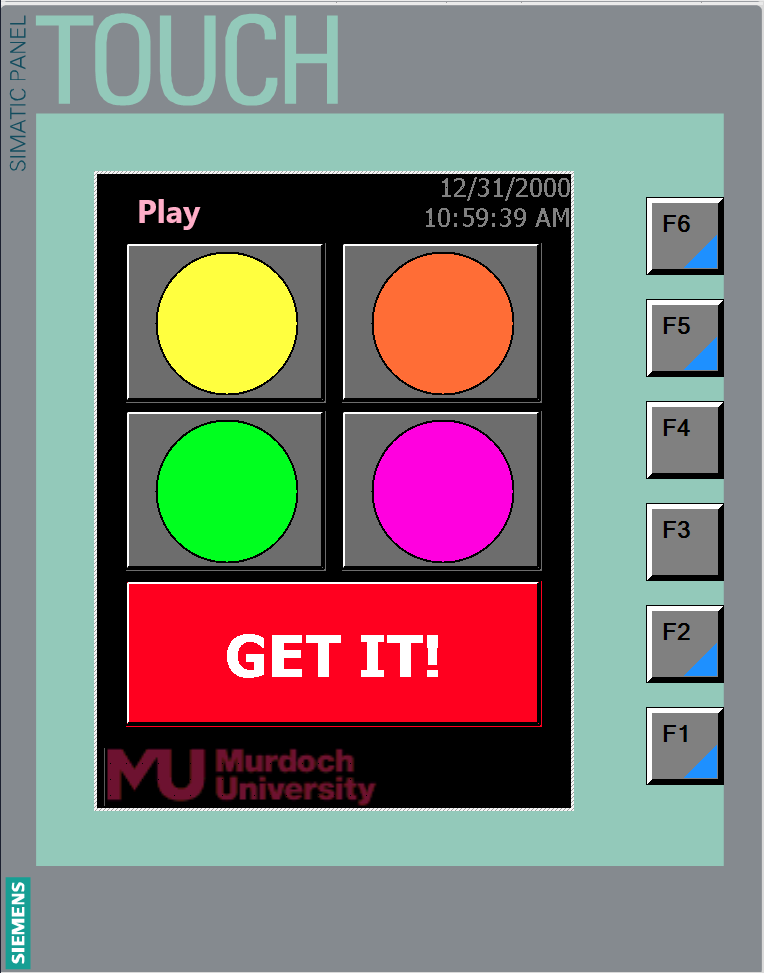
\includegraphics[width = 0.3\textwidth]{2_images/hmiPlay}
            \caption{The Play screen on the Siemens HMI}
            \label{fig:hmiPlay}
        \end{figure} 

        \subsubsection{Home}
            The home page is the main screen from a machine operations and maintenance perspective. This screen allows the operator to control and monitor the machine mode and control source - it also provides navigation to other screens. This screen can be accessed by at any time by pressing F1.  
        
        \begin{figure}[H]
            \centering
            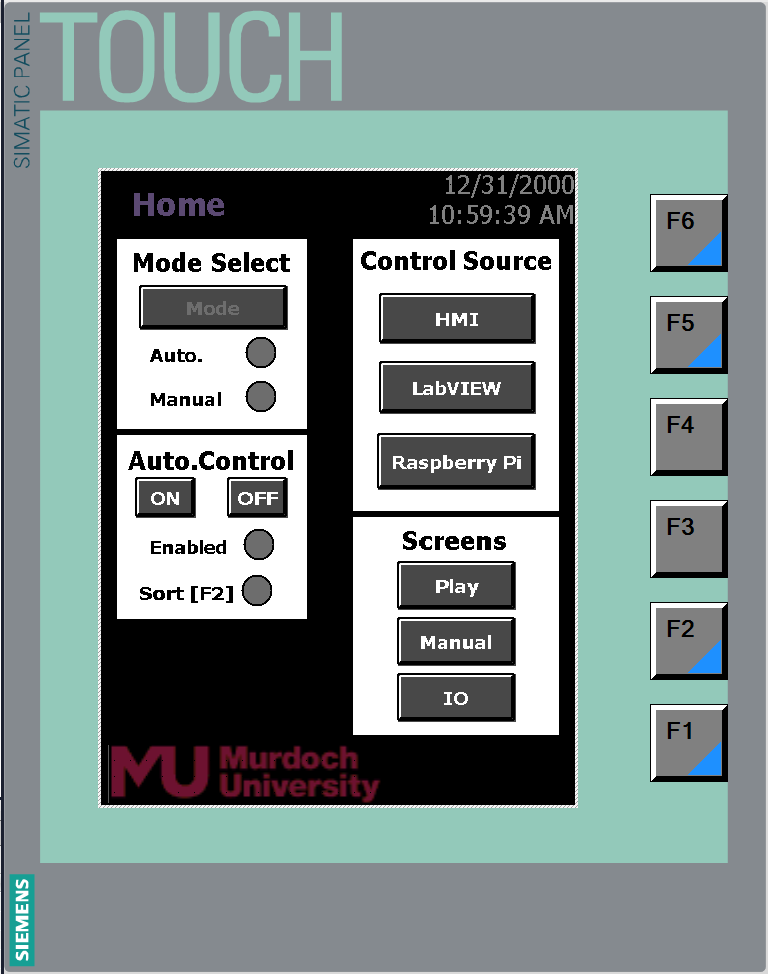
\includegraphics[width = 0.3\textwidth]{2_images/hmiHome.png}
            \caption{The home screen on the Siemens HMI}
            \label{fig:hmiHome}
        \end{figure} 
        
        \subsubsection{Manual}
            This screen provides manual operation to all valves. To change the state of a valve in manual mode, simply press the Vn button. When the valve is switched on the grey button will change color to green. This screen is accessible by pressing the manual button on the home screen. 

        \begin{figure}[H]
            \centering
            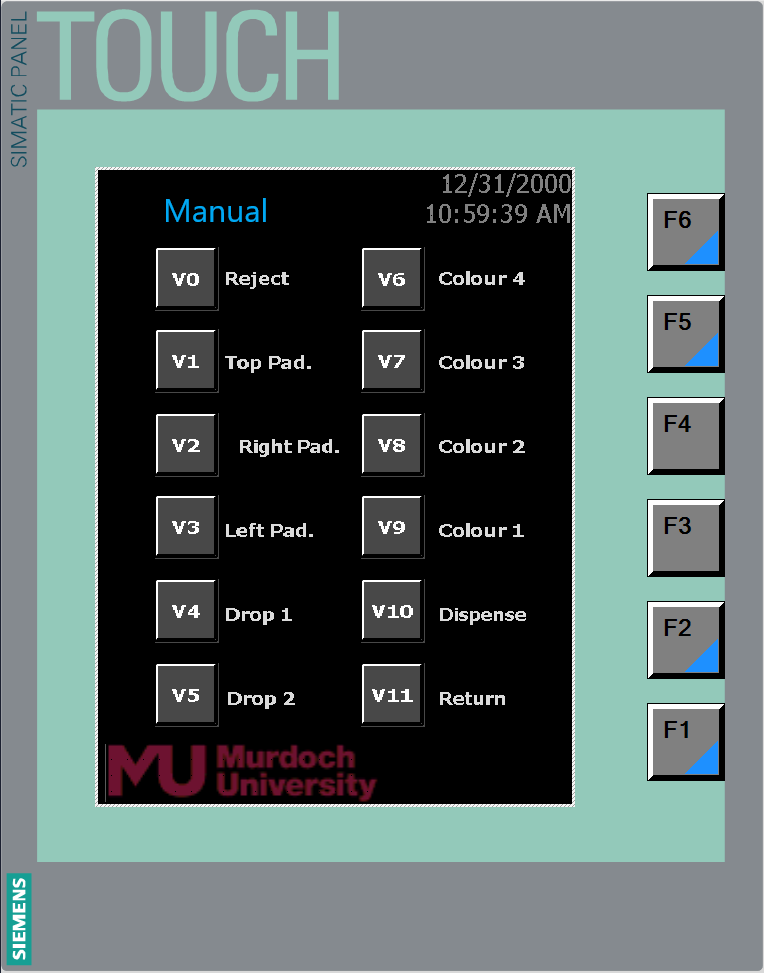
\includegraphics[width = 0.3\textwidth]{2_images/hmiManual}
            \caption{The manual screen on the Siemens HMI}
            \label{fig:hmiManual}
        \end{figure} 

        \subsubsection{IO}
            This screen shows machine \acrshort{io} status. This screen can be used as a diagnostic tool for machine operators. The \acrshort{io} screen also provides an impressive representation of the events occurring while the sorting program is running and users are dispensing lollies. This screen will show the \acrshort{io} status regardless of which control source is active.   

            \begin{description}
                \item Grey = False
                \item Green = True
            \end{description}

        \begin{figure}[H]
            \centering
            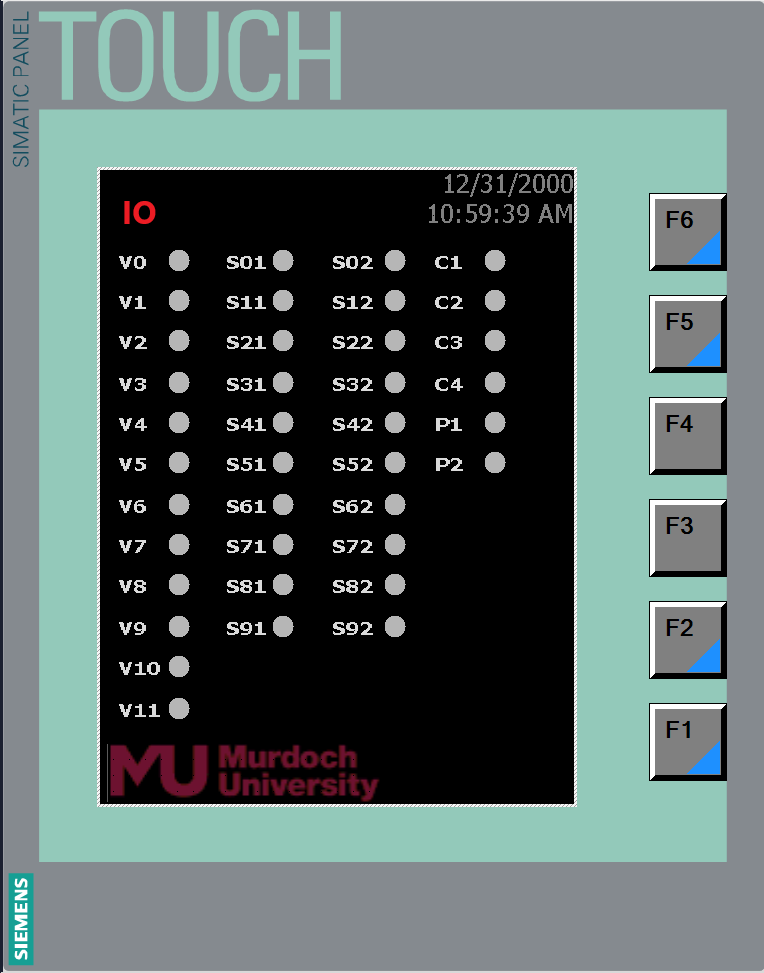
\includegraphics[width = 0.3\textwidth]{2_images/hmiIo}
            \caption{The io screen on the Siemens HMI}
            \label{fig:hmiIo}
        \end{figure} 
    
\section{LabVIEW}
    A LabVIEW application to control and monitor the lolly machine has also been developed. This interface has been built with an intuitive design to allow operators to easily troubleshoot and diagnose problems. The LabVIEW application was the quickest to develop as functions from inbuilt libraries were used for most programming tasks.

    While developing with LabVIEW, the front and back panel are developed at the same time - this makes development comparatively quick.
    
    \subsection{Back Panel}
    
        The back panel of the LabVIEW program contains program logic and functions that drive the application. 
        
        \subsubsection{Modbus Communication}
        
            Modbus communication functions from \href{https://www.ni.com/en-au/support/downloads/tools-network/download.modbus-master.html#374378}{Modbus Master by Plasmionique Inc.} made configuring and programming Modbus components a uncomplicated task \cite{modbusLabview}.
            
            Establishing a connection to the \acrshort{plc} is accomplished through a Modbus master function which requires the \acrshort{ip} address and port number of the Modbus server - the \acrshort{plc}(192.168.1.10). 
            Read functions (reading glasses) are used to read values form the Modbus Server while write functions (pencil), write values to the Server. Address indexing in LabVIEW starts at zero while the \acrshort{plc} starts at one, this means that an offset of one exists between Modbus addresses of the \acrshort{plc} and the LabVIEW application. Figure\ref{fig:modLabFun}
            
        \begin{figure}[H]
            \centering
            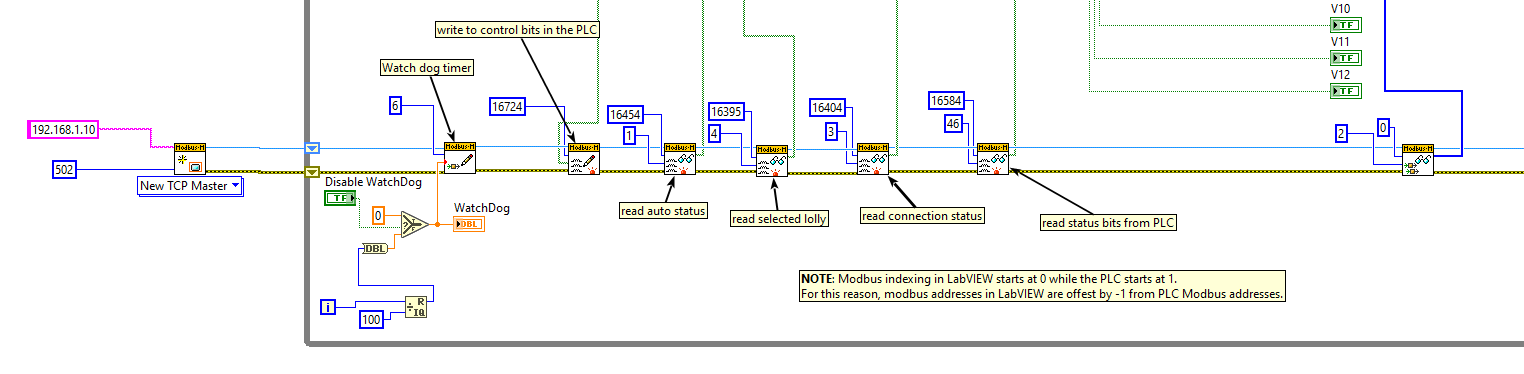
\includegraphics[width = 0.9\textwidth]{2_images/labViewModFunc}
            \caption{The Modbus functions on the LabVIEW back panel.}
            \label{fig:modLabFun}
        \end{figure}     
        
        \subsubsection{Watch Dog Timer}
            Building a watchdog timer with LabVIEW was a simple task with the core components being the loop iteration number and a quotient/ remainder function. An additional feature is added to the watchdog timer that allows users to pause the timer. This feature is included to simulate a disconnection, thus, demonstrating the  previously discussed automatic control source recovery function (Section \ref{sec:autoConRec}).

        \begin{figure}[H]
            \centering
            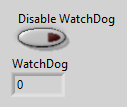
\includegraphics[width = 0.2\textwidth]{2_images/labFrontWatchDog}
            \caption{The LabVIEW watchdog indicator.}
            \label{fig:labFrontWatchDog}
        \end{figure}    
            
            
        \subsubsection{Data Conversion}
            To read data from the \acrshort{plc}, data needed to be converted from a Boolean array into individual bits, and vice versa for writing. This was achieved in LabVIEW using standard array functions found in the main tool palette. Converting the alarm words into individual bits was accomplished through a few different functions. An array of 16 bit integers is split into two separate integers. Each integer is then converted into bits which are connected to Boolean indicators. This flow of conversions is illustrated in Figure \ref{fig:labViewAlarmUnmap}.

        \begin{figure}[H]
                \centering
                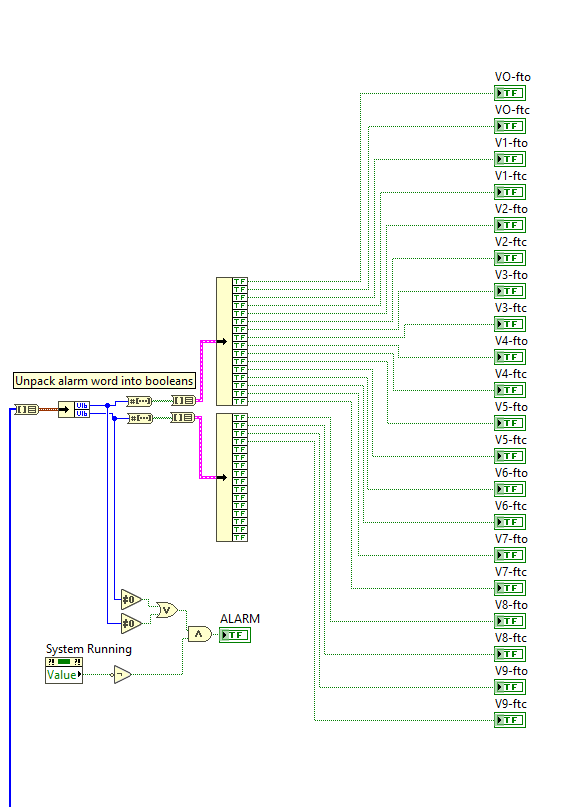
\includegraphics[width = 0.4\textwidth]{2_images/labViewAlarmUnmap}
                \caption{Unmapping alarm words with LabVIEW.}
                \label{fig:labViewAlarmUnmap}
        \end{figure}   
            
        \subsubsection{Front Panel}

            The front panel of the LabVIEW application is what the users interact with.
            
            The LabVIEW front panel for this project has been designed to look like the machine. The intention behind this was to make troubleshooting and diagnostics activities more intuitive and therefore a quicker and easier. Although LabVIEW has the capability to build complicated screens with multiple tabs and pages, a deliberate effort was made to make the front panel a single page without any tabs (except for those incorporated into the `how to' section).
            
            Indicators on the machine graphic allow users to easily see the \acrshort{io} status of the machine. Linear actuators are replicated by the blue rectangles, the colour of the valve indicator within the rectangles signify the position of the actuator. 
            Rotary actuators are the three V shapes above the secondary hoppers. The colour of the indicator at the bottom of each V is associated with the position of each colour paddle.
            Valve graphics for V11 and V12 change colour to green when they are turned on. Valve position switches on the right of the panel turn bright green when True and dark green when False. 

            The right hand side of the panel is where users are able to interact with the machine. Status indicators in the control source box show where the \acrshort{plc} is being controlled from. The `Request Control' button diverts the control to the LabVIEW application. Automatic and manual control can also be achieved from the LabVIEW program. 

            When an alarm is active, the indicator associated with the specific alarm will go red and the large alarm indicator will flash. 

            As a side note, the lollies in the primary hopper shown on the front panel are for aesthetic purposes only and do not have any relation to what is currently in the machine. 

        \begin{figure}[H]
                \centering
                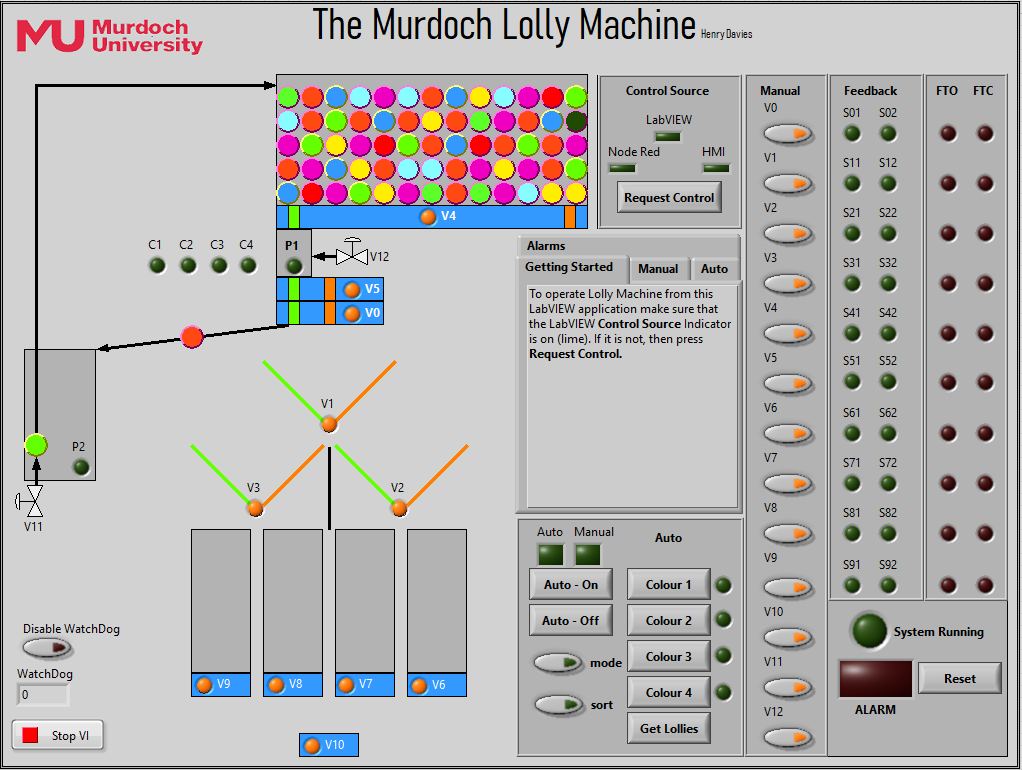
\includegraphics[width = 0.6\textwidth]{2_images/labViewFrontOverview}
                \caption{The LabVIEW front panel in all its glory.}
                \label{fig:abViewFrontOverview}
        \end{figure}               


\section{Raspberry-Pi/ Node-RED}
    Node-RED is a programming tool that links hardware devices, \acrshort{api}s and online services through a method called a program flow \cite{nodeRed}. For this project, Node-RED is hosted on a Raspberry Pi Microcontroller and is used to link WiFi enabled devices (smart phones, tablets, computers, etc) to the lolly machine.

    \subsection{Raspberry Pi}
        The Raspberry Pi used in this project has been configured as a \acrshort{wap} to allow a remote connection from WiFi enabled devices. Setting up the \acrshort{wap} was achieved by following a step by step method found \href{https://raspberrypi-guide.github.io/networking/create-wireless-access-point}{online}\cite{wapSetup}. The WiFi credentials are as follows:
        
        \begin{description}
            \item WiFi Name = Lolly Machine
            \item Password  = iwantcandy 
        \end{description}

        The Raspberry Pi is installed in the backside of the lolly machine inside an Phoenix Contact industrial din mount housing. See Figure \ref{fig:raspPiInstall}.
              
    \subsection{Node-RED Flow}
        Node-RED flows consist of multiple nodes connected to one another with wires. Nodes are the fundamental building blocks which send and/or receive data from other nodes within the flow. To access the Node-RED flow, connect to the Raspberry Pi through the WiFi or Ethernet network and go to the following web address:
        \newline\textit{192.168.1.120:1880}
        The Node-RED flow is illustrated in Figure \ref{fig:nodeRedFlow}.
        \begin{figure}[H]
            \centering
            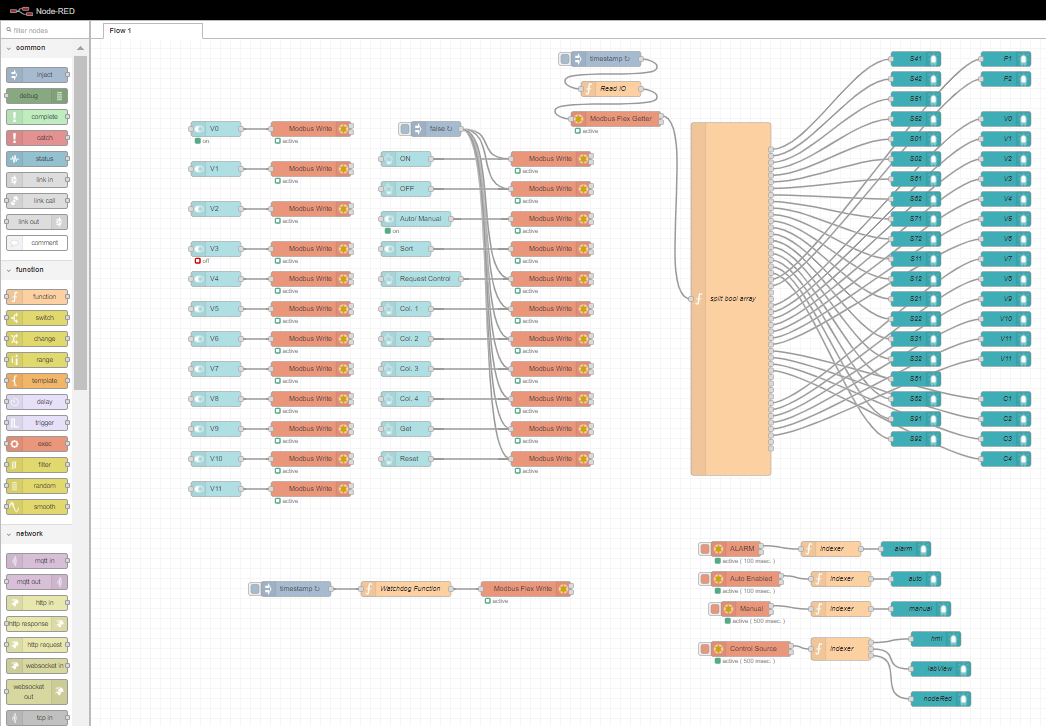
\includegraphics[width = 0.85\textwidth]{2_images/nodeRedFlow}
            \caption{The Node-RED flow.}
            \label{fig:nodeRedFlow}
        \end{figure}  
        
        \subsubsection{Modbus Communication}
            A Node-RED Modbus library, containing Modbus functions, must be added to the Node-RED service as it does not come with the default download. To download the Modbus library onto the Raspberry Pi, the following command must be run in the terminal window of the Raspberry Pi. \newline\textit{npm install node-red-contrib-Modbus}\footnote{The Raspberry Pi must be connected to the Internet.} \newline
            Once this is complete, a set of Modbus function nodes become available for use. This project only required the use of a few different functions. Writing to Modbus addresses on the \acrshort{plc} is achieved with `Modbus Write' functions. Modbus write functions receive Boolean data from dashboard inputs and are configured with their associated \acrshort{plc} address. Read addresses are read by a `Modbus Flex Getter' node which requires the configuration data to be passed into it by its preceding node. The configuration parameters passed into the node can be seen below in Listing \ref{list:modGetCon} which reads 46 Modbus coil addresses starting from Modbus address 16584.

            \begin{lstlisting}[language=Java, caption = Configuration for Modbus Flex Getter, label=list:modGetCon]
                msg.payload = {
                    value: msg.payload,
                    'fc': 1,
                    'unitid': 1,
                    'address':16584,
                    'quantity':46}
                return msg;
            \end{lstlisting}
            
            The `Modbus Flex Getter' function returns a Boolean array which needs to be split and wired into dashboard indicators - this is achieved through a custom function as seen in Listing \ref{list:splitBolArr}.
            
            \begin{lstlisting}[language=Java, caption = Javascript to split Boolean array, label=list:splitBolArr]
                // create empty array 
                nvar outArr = []
                // move msg.payload into 'input' variable
                nvar input = msg.payload
                // find array length
                nvar arrLen = input.length
                //build array of payload objects with values from input
                for ( var n = 0; n < 47 ; n++){
                    outArr.push({ payload: input[n] })
                	}
                return outArr ;
            \end{lstlisting}
            
            
            Extra detail on using Modbus with Node-RED can be found online on this \href{https://stevesnoderedguide.com/node-red-modbus}{link} \cite{modbusNodeRed}.
            
        \subsubsection{Watch Dog Timer}
            A watchdog timer has been implemented using the UNIX type timestamp node. A function has been written that passes the timestamp data so that only the seconds are being sent to the Modbus Function (Listing \ref{fig:nodeRedWatchDogFlow}). This flow is illustrated in Figure \ref{fig:nodeRedWatchDogFlow}

            \begin{figure}[H]
                    \centering
                    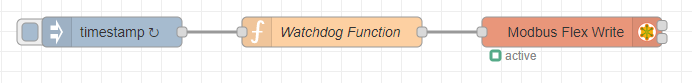
\includegraphics[width = 0.85\textwidth]{2_images/nodeRedWatchDogFlow}
                    \caption{Node flow for the watchdog timer.}
                    \label{fig:nodeRedWatchDogFlow}
            \end{figure}  


            \begin{lstlisting}[language=Java, caption=Watchdog timer script, label=list:watchDog]
                var input = msg.payload
                var str1 = input.toString()
                var str2 = str1.slice(8,11)
                var num = Number(str2)
                var fc = 6;
                var sa = 8;
                var addresses = 7;
                var value = num;
                msg.slave_ip = "192.168.1.10";
                msg.payload = { "value": value, 'fc': fc, 'unitid': 1, 
                'address': sa, 'quantity': addresses };
                return msg;
            \end{lstlisting}            

    \subsection{Node-RED Dashboard}
        The Node-RED dashboard is configured in the Node-RED flow space and accessible on devices connected to the Raspberry Pi through the following web address. \newline \textit{192.168.1.120:1880/ui} \newline The dashboard has two tabs, one that provides the status of the machine and other for control. The status tab shows machine \acrshort{io} status through indicators which are green when true and grey when false. The Node-RED dashboard, unlike the other control sources, does not display specific alarm details however, 
        The control tab provides an interface that allows users to remotely control the machine. Functionality from the Node-RED dashboard is the same as the other control sources. Instructions on how to use the dashboard can be found in the user manual (Appendix \ref{app:userGuide}).

        \begin{figure}[H]
            \centering
            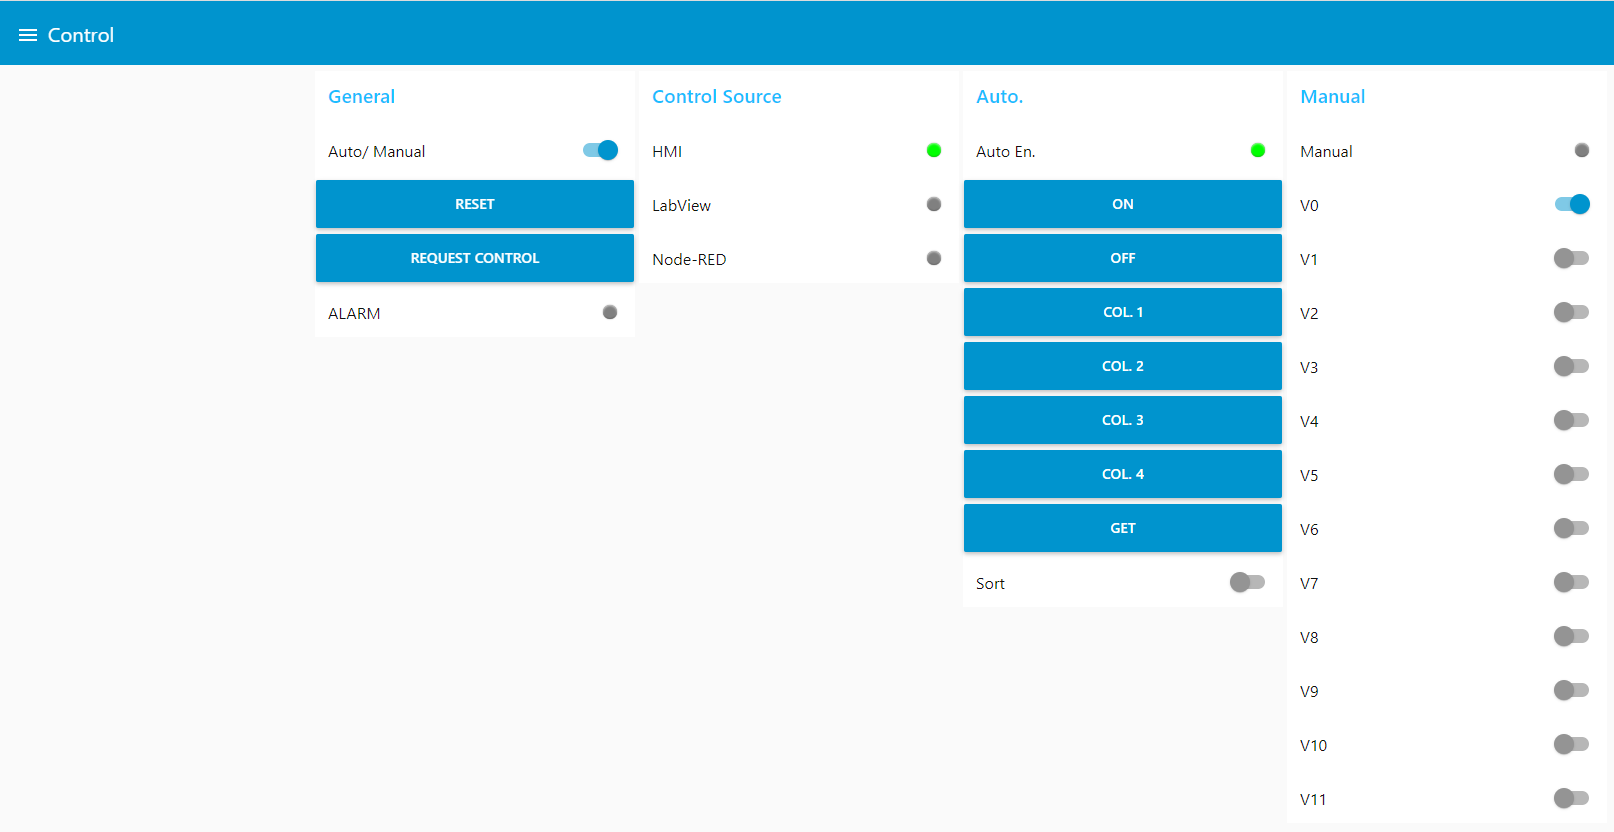
\includegraphics[width = 0.85\textwidth]{2_images/nodeRedControl}
            \caption{The Node-RED control dashboard.}
            \label{fig:nodeRedControl}
        \end{figure}  
        
\section{Physical Push Buttons and LED Indicators}
    Although the physical push buttons and \acrshort{led}s are not by definition a \acrshort{hmi}, they are included as they do serve as a low level interface between the user and machine.

    \subsubsection{Dispense Function}
        Five push buttons on the lower half of the front panel are linked directly to the dispense function. Four buttons on the right are for lolly selection, while the one on the left will execute the function. All buttons have \acrshort{led} feedback indicators. The colour selection buttons will only illuminate when the associated colour is selected - illumination will occur regardless of where the machine is being controlled from. The execute button will illuminate whenever pressed.

        \begin{figure}[H]
            \centering
            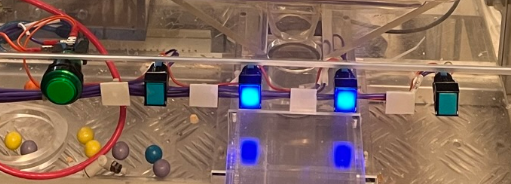
\includegraphics[width = 0.85\textwidth]{2_images/physicalPushButtons}
            \caption{Physical push buttons for the dispensing function.}
            \label{fig:physicalPushButtons}
        \end{figure}          

    \subsubsection{Traffic Light Indicators}
        Three \acrshort{led}s located on the top left of the front panel provide machine status information. The \acrshort{led}s are installed in a traffic light configuration. 

        \begin{description}
            \item[Red Solid:] Alarm Mode. When in this state the machine will not run. 
            \item Amber Solid: Manual Mode.
            \item Green Flashing: Automatic Mode - Not Enabled
            \item Green Solid: Automatic Mode - Enabled
        \end{description}
        
    
    
